\chapter{Dynamics in the thermodynamic limit}\label{ch:mean_field_analysis}
\section{The importance of local pumping}
At this point I want to emphasize that local pumping is crucial for the occurrence of non trivial long-time behavior. In the absence of this local pumping the system decays to the fully mixed state. To see this it is helpful to look at the properties of the total spin.
\begin{align}
    m^2\vcentcolon&=m_x^2+m_y^2+m_z^2\notag\\
    \Rightarrow\quad\dt m^2&=2\,\left( m_x\,\dt m_x +m_y\,\dt m_y +m_z\,\dt m_z \right)\notag\\
    &=-\vec{m}^t\,\left( \begin{array}{ccc}
        \Gamma+\gamma & 0&0  \\
        0& \Gamma+\gamma & 0\\
        0&0&2\,\Gamma
   \end{array}\right)\,\vec{m}+\Gamma\,m_z\notag\\
   &=-\left(  (\Gamma+\gamma)\,(m_x^2+m_y^2)+2\,\Gamma\,m_z^2-\Gamma\,m_z \right)
\end{align}
Because in the case $\Gamma=0$ the derivative of $|m|^2$ reduces to the matrix scalar product, the derivative is always negative for positive definite matrices.  In \appref{appendix:msq_calc} it is shown that in our case the semi-positive definiteness of the matrix is sufficient for the general decay. From this expression can also be told that laser driving, detuning and collective spontaneous emission have no direct influence on the total spin modulus.

\section{Zero detuning case}\label{sec:zero_detuning}
\subsection{Analysis of the fixed points}
One of the most interesting characteristics of a system is its long-time behavior. A key point of such analysis is the determination of stationary points, where a certain configuration of the collective spin does not change in time. Those fixed points of the time propagation are, if they are stable, the configuration, at whom at least part of the system arrives for long times. \\
This is why I first examine the solutions that set the right hand side of the equations of motion to zero. i.e. $\text{d}m_x/\text{d}t=\text{d}m_y/\text{d}t=\text{d}m_z/\text{d}t=0$. As a consequence the $m_z$-equation can be expressed via
\begin{align}
    m_z=\half-\frac{1}{\Gamma}\,\left(\kappa\,(m_x^2+ m_y^2)-\omega\,m_y  \right)
\end{align}
in the case $\Gamma\neq0$. This makes the problem 2 dimensional. After substituting $m_z$ in the remaining two equations of motion and multiplying the equations with $2\Gamma$, one arrives at
% \begin{align*}
%     -\frac{\delta}{2}\,m_y-\half\,(\gamma+\Gamma)\,m_x+\kappa\,m_x\,\left( \half-\frac{1}{\Gamma}\,\left(\kappa\,(m_x^2+ m_y^2)-\omega\,m_y  \right)  \right)&=0\\
%     \frac{\delta}{2}\,m_x-\omega\,\left( \half-\frac{1}{\Gamma}\,\left(\kappa\,(m_x^2+ m_y^2)-\omega\,m_y  \right)  \right)&\\-\half\,(\gamma+\Gamma)\,m_y+\kappa\,m_y\,\left( \half-\frac{1}{\Gamma}\,\left(\kappa\,(m_x^2+ m_y^2)-\omega\,m_y  \right)  \right)&=0\\\\
%     \text{multiplying with }2\Gamma\text{ yields}\quad\quad\quad\hspace*{6cm}&
%     \\\Rightarrow\quad
\begin{align}-\Gamma\delta\,m_y-\Gamma\,(\gamma+\Gamma-\kappa)\,m_x-2\,\kappa^2\,m_x\,( m_x^2+ m_y^2)+2\,\kappa\omega\,m_xm_y  &=0\notag\\\notag\\
    \Gamma\delta\,m_x-\omega\Gamma-\Gamma\,(\gamma+\Gamma-\kappa+2\,\omega^2/\Gamma)\,m_y&\notag\\
    -2\,\kappa^2\,m_y\,( m_x^2+ m_y^2)+2\,\kappa\omega\,(m_x^2+2\,m_y^2)  &=0
\end{align}
In the following I set $\delta=0$. This simplification makes a analytical examination possible, allowing me to get a deeper intuition of some key features, regarding systems of this type. 
A series of rescaling processes are helpful, in order to make the equations of motion cleaner. With the definition $\omega=\tilde{\omega}/\sqrt{2}$, $\kappa=\tilde{\kappa}/\sqrt{2}$ and $\Gamma+\gamma-\tilde{\kappa}/\sqrt{2}=\vcentcolon \tilde{A}\tilde{\kappa}^2$, the stationary solutions are determined by
\begin{align*}
    -m_x\,\left(\Gamma\tilde{A}+( m_x^2+ m_y^2)-\frac{\tilde{\omega}}{\tilde{\kappa}}\,m_y\right)  &=0\\\\
    -\frac{\tilde{\omega}\Gamma}{\sqrt{2}\,\tilde{\kappa}^2}-\Gamma\tilde{A}\,m_y    -m_ym_x^2- m_y^3+\frac{\tilde{\omega}}{\tilde{\kappa}}\,(m_x^2+2\,m_y^2)-\frac{\tilde{\omega}^2}{\tilde{\kappa}^2}\,m_y  &=0
\end{align*}
The first equation can be dropped in the future, because the only solution of this system is found at $m_x=0$. A solution $m_x\neq0$ would require
\begin{align*}
    m_x^2&=-m_y^2+\frac{\tilde{\omega}}{\tilde{\kappa}}\,m_y-\Gamma\tilde{A} \\
    \Rightarrow\quad0&=-\frac{\tilde{\omega}\Gamma}{\sqrt{2}\,\tilde{\kappa}^2}-\Gamma\tilde{A}\,m_y    -m_y\,(-m_y^2+\frac{\tilde{\omega}}{\tilde{\kappa}}\,m_y-\Gamma\tilde{A})- m_y^3+\frac{\tilde{\omega}}{\tilde{\kappa}}\,(-m_y^2+\frac{\tilde{\omega}}{\tilde{\kappa}}\,m_y-\Gamma\tilde{A}+2\,m_y^2)-\frac{\tilde{\omega}^2}{\tilde{\kappa}^2}\,m_y  \\
    &=-\frac{\tilde{\omega}\Gamma}{\sqrt{2}\,\tilde{\kappa}^2}-\frac{\tilde{\omega}}{\tilde{\kappa}}\,\Gamma\tilde{A}\\
    &=-\frac{1}{\sqrt{2}\,\tilde{\kappa}}-\frac{1}{\tilde{\kappa}^2}\,(\Gamma+\gamma-\frac{\tilde{\kappa}}{\sqrt{2}})=-\frac{1}{\tilde{\kappa}^2}\,(\Gamma+\gamma)
\end{align*} 
For $\Gamma,\,\gamma\neq0$, it can not be satisfied. As mentioned earlier this is the case, in which this project is interested in. So the only possible stationary solutions are
\begin{align*}
    m_x&=0\\
    m_y&=\ty\\
    \text{with}\quad0&=-\frac{\tilde{\omega}\Gamma}{\sqrt{2}\,\tilde{\kappa}^2}-\Gamma\tilde{A}\,\ty    - \ty^3+2\,\frac{\tilde{\omega}}{\tilde{\kappa}}\,\ty^2-\frac{\tilde{\omega}^2}{\tilde{\kappa}^2}\,\ty  
\end{align*}
% One can multiply the equation with $\tilde{\kappa}^3/\tilde{\omega}^3$ in order to receive
% \begin{align*}
%     0&=-\frac{\tilde{\kappa}\Gamma}{\sqrt{2}\,\tilde{\omega}^2}-(\frac{\tilde{\kappa}^2}{\tilde{\omega}^2}\,\Gamma\tilde{A}+1)\,\frac{\tilde{\kappa}}{\tilde{\omega}}\,\ty    - \frac{\tilde{\kappa}^3}{\tilde{\omega}^3}\,\ty^3+2\,\frac{\tilde{\kappa}^2}{\tilde{\omega}^2}\,\ty^2 
% \end{align*}
Multiplying with $\tilde{\kappa}^3/\tilde{\omega}^3$ and redefining ${y}\vcentcolon=\ty\tilde{\kappa}/\tilde{\omega}$ and $\Gamma A\vcentcolon=\tilde{\kappa}^2/\tilde{\omega}^2\,\Gamma\tilde{A}$ the stationary solutions are determined by a cleaner expression, i.e.
\begin{align}
    m_x&=0\notag\\
    m_y&=\tilde{\omega}/\tilde{\kappa}\,{y}\notag\\
    \text{with}\quad0&=-B-(\Gamma A+1)\,{y}    - {y}^3+2\,{y}^2=\vcentcolon F({y})\notag\\
    \text{with}\quad B\vcentcolon&= \frac{\tilde{\kappa}\Gamma}{\sqrt{2}\,\tilde{\omega}^2}
\end{align}
First I want to examine the number of stationary solutions the system possesses. The polynomial of third degree, determining the $y$-value of the fixed point, can have at most two extrema. Only in this case the function is not monotone and can have more than one root. The derivative of $F$ with respect to $y$ reads
\begin{align*}
    F'(y)=-\Gamma A-1 -3\,y^2+4\,y
\end{align*}
It has its roots at the positions
\begin{align*}
    y_{12}=&\frac{1}{3}\,\left(  2\pm \sqrt{4-3\,(\Gamma A+1)}  \right)\\
    =&\frac{1}{3}\,\left(  2\pm \sqrt{1-3\,\Gamma A}  \right)
\end{align*}
Hence $F(y)$ has no extrema, if $\Gamma A\geq1/3$. Through the choice of the parameters $\Gamma A$ the position and existence of the roots can be controlled. By resolving the above equation for $\Gamma A$, 
\begin{align*}
    % (3\,y_{12}-2)^2=&1-3\,\Gamma A\\
    \Gamma A=& \frac{1}{3}\,\left(  1-(3\,y_{12}-2)^2 \right)
\end{align*}
and inserting it into $F$, the value of the extrema at $y_{12}$ is located at
\begin{align*}
    F(y_{12})=&%-B-\frac{1}{3}\,\left(  1-(3\,y_{12}-2)^2 +3\right)\,y_{12}-y_{12}^3+2\,y_{12}^2\\
    %=&-B-\frac{1}{3}\,\left( - 9\,y_{12}^2+12\,y_{12}\right)\,y_{12}-y_{12}^3+2\,y_{12}^2\\
    -B+2\,y_{12}^3-2\,y_{12}^2
\end{align*}
$F(y_{12})$ gives the value of the maximum and minimum of $F$. For $B=0$ there remains
\begin{align*}
    F(y_{12})=&2\,y_{12}^3-2\,y_{12}^2\\
    =&2\,y_{12}^2\,(y_{12}-1)
    %&=\vcentcolon F_\text{max}(y_{12})
\end{align*}
One can tell from here, that the maximum is negative until $y_{12}=1$ which corresponds to $\Gamma A =0$ and the minimum is always negative except when $y_{12}=0$ which corresponds to $\Gamma A=-1$ and $B=0$. The saddle point of the polynomial is located at the configuration $\Gamma A=1/3$ and $y=2/3$. As has just been seen the maximum and minimum, which fall together at this point, lie for $y=2/3$ below zero. Therefore, no value of $B>0$ can be taken such that the saddle point becomes a stationary solution.  
\begin{figure}[H]
    \centering
    \caption{The determining function $F(y)$ is plotted for different values of $\Gamma A$, while $B$ is set to zero. A non-zero $B$-value would shift the polynomials down.}
    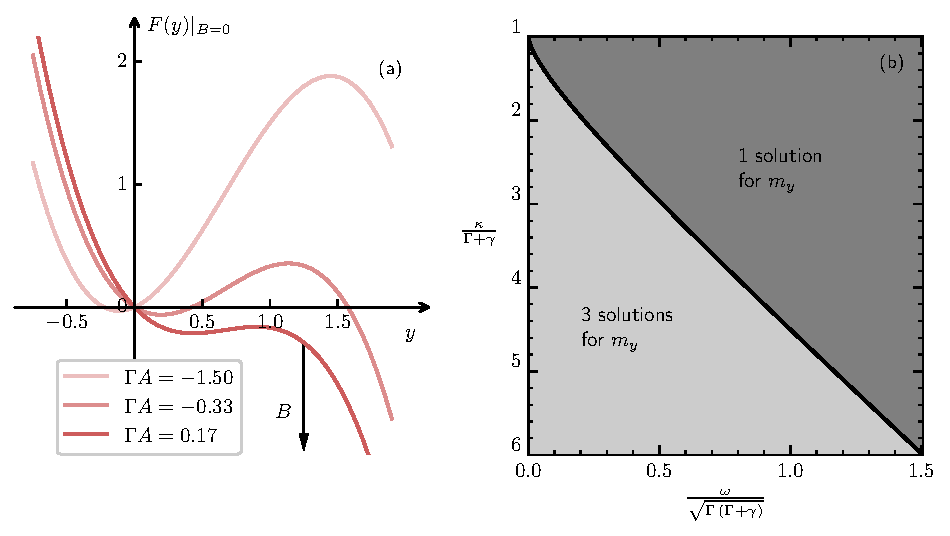
\includegraphics{pictures/polynomial_scheme_phase.pdf}
    \label{fig:numb_fixp}
\end{figure}
For sufficiently large values of $B$, the function is shifted downwards such that only one root survives. Consequently there is a critical constellation of $B$, so that the number of solutions change from one to three. This idea can be made advantage of for calculating the number of fixed points. If the local maximum of $F$ lies below zero, only one root exists.
% \begin{wrapfigure}[19]{l}{0pt}
%     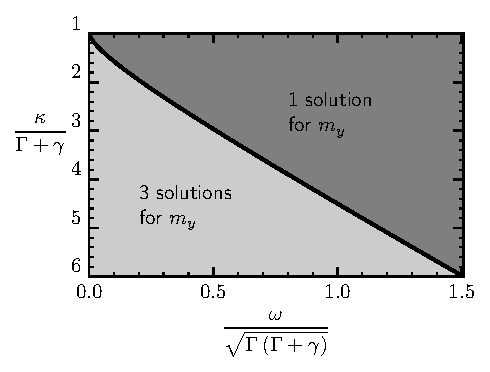
\includegraphics{pictures/numb_fixp2.pdf}
%     \vspace*{-2cm}\caption{The number of fixed points depending on the parameter configuration.}
%     \label{fig:numb_fixp}
% \end{wrapfigure}
With the rescaling $\Omega=\tw/\sqrt{2\,\Gamma\,(\Gamma+\gamma)}$ and $K=\tk/(\sqrt{2}\,(\Gamma+\gamma))$ one gets
\begin{gather*}
    B=\frac{K}{2\,\Omega^2}\\\text{and}\quad
% \end{align*}
% and
% \begin{align*}
    y_\text{max}=\frac{1}{3}\,\left( 2+ \sqrt{1-\frac{3}{2}\,(1-K)\,\frac{1}{\Omega^2}}  \right)
\end{gather*}
and thus the problem only depends on two parameters. Now the border between the configurations with different numbers of fixed points can be determined, by numerically meeting the above mentioned condition of a local maximum with $F(y_{12})=0$. To be explicit this is done by calculating the root of $F(y_{12})$ with respect to $K$ for various values of $\Omega$. The result is shown in \figref{fig:numb_fixp}\\\\As known from previous considerations if $y_\text{max}<1$, i.e. $A>0$ which corresponds to $K>1$, the maximum of $F$ is negative even for $B=0$, resulting in only one solution. Another thing can be noted at this point. As $F(0)=-B$ and $B\neq0$ for $\kappa\neq0$, one solution $m_y$ has always to be negative for $\kappa\neq0$.\\\\

As stable fixed points are possible long-time states of the system, it would be possibly problematic, if they lied outside the physically allowed space, meaning $|m|\leq1/2$. Reassuringly this is never the case as I show in \appref{appendix:mod_of_fixp}. Numerical calculations deliver the same result. I want to mention at this point that in all diagrams that are shown in this thesis $\Gamma=1$ is chosen. All coupling strengths, i.e. energies, are measured in the units of $\Gamma=1$. %
% \begin{wrapfigure}[22]{l}{0pt}
%     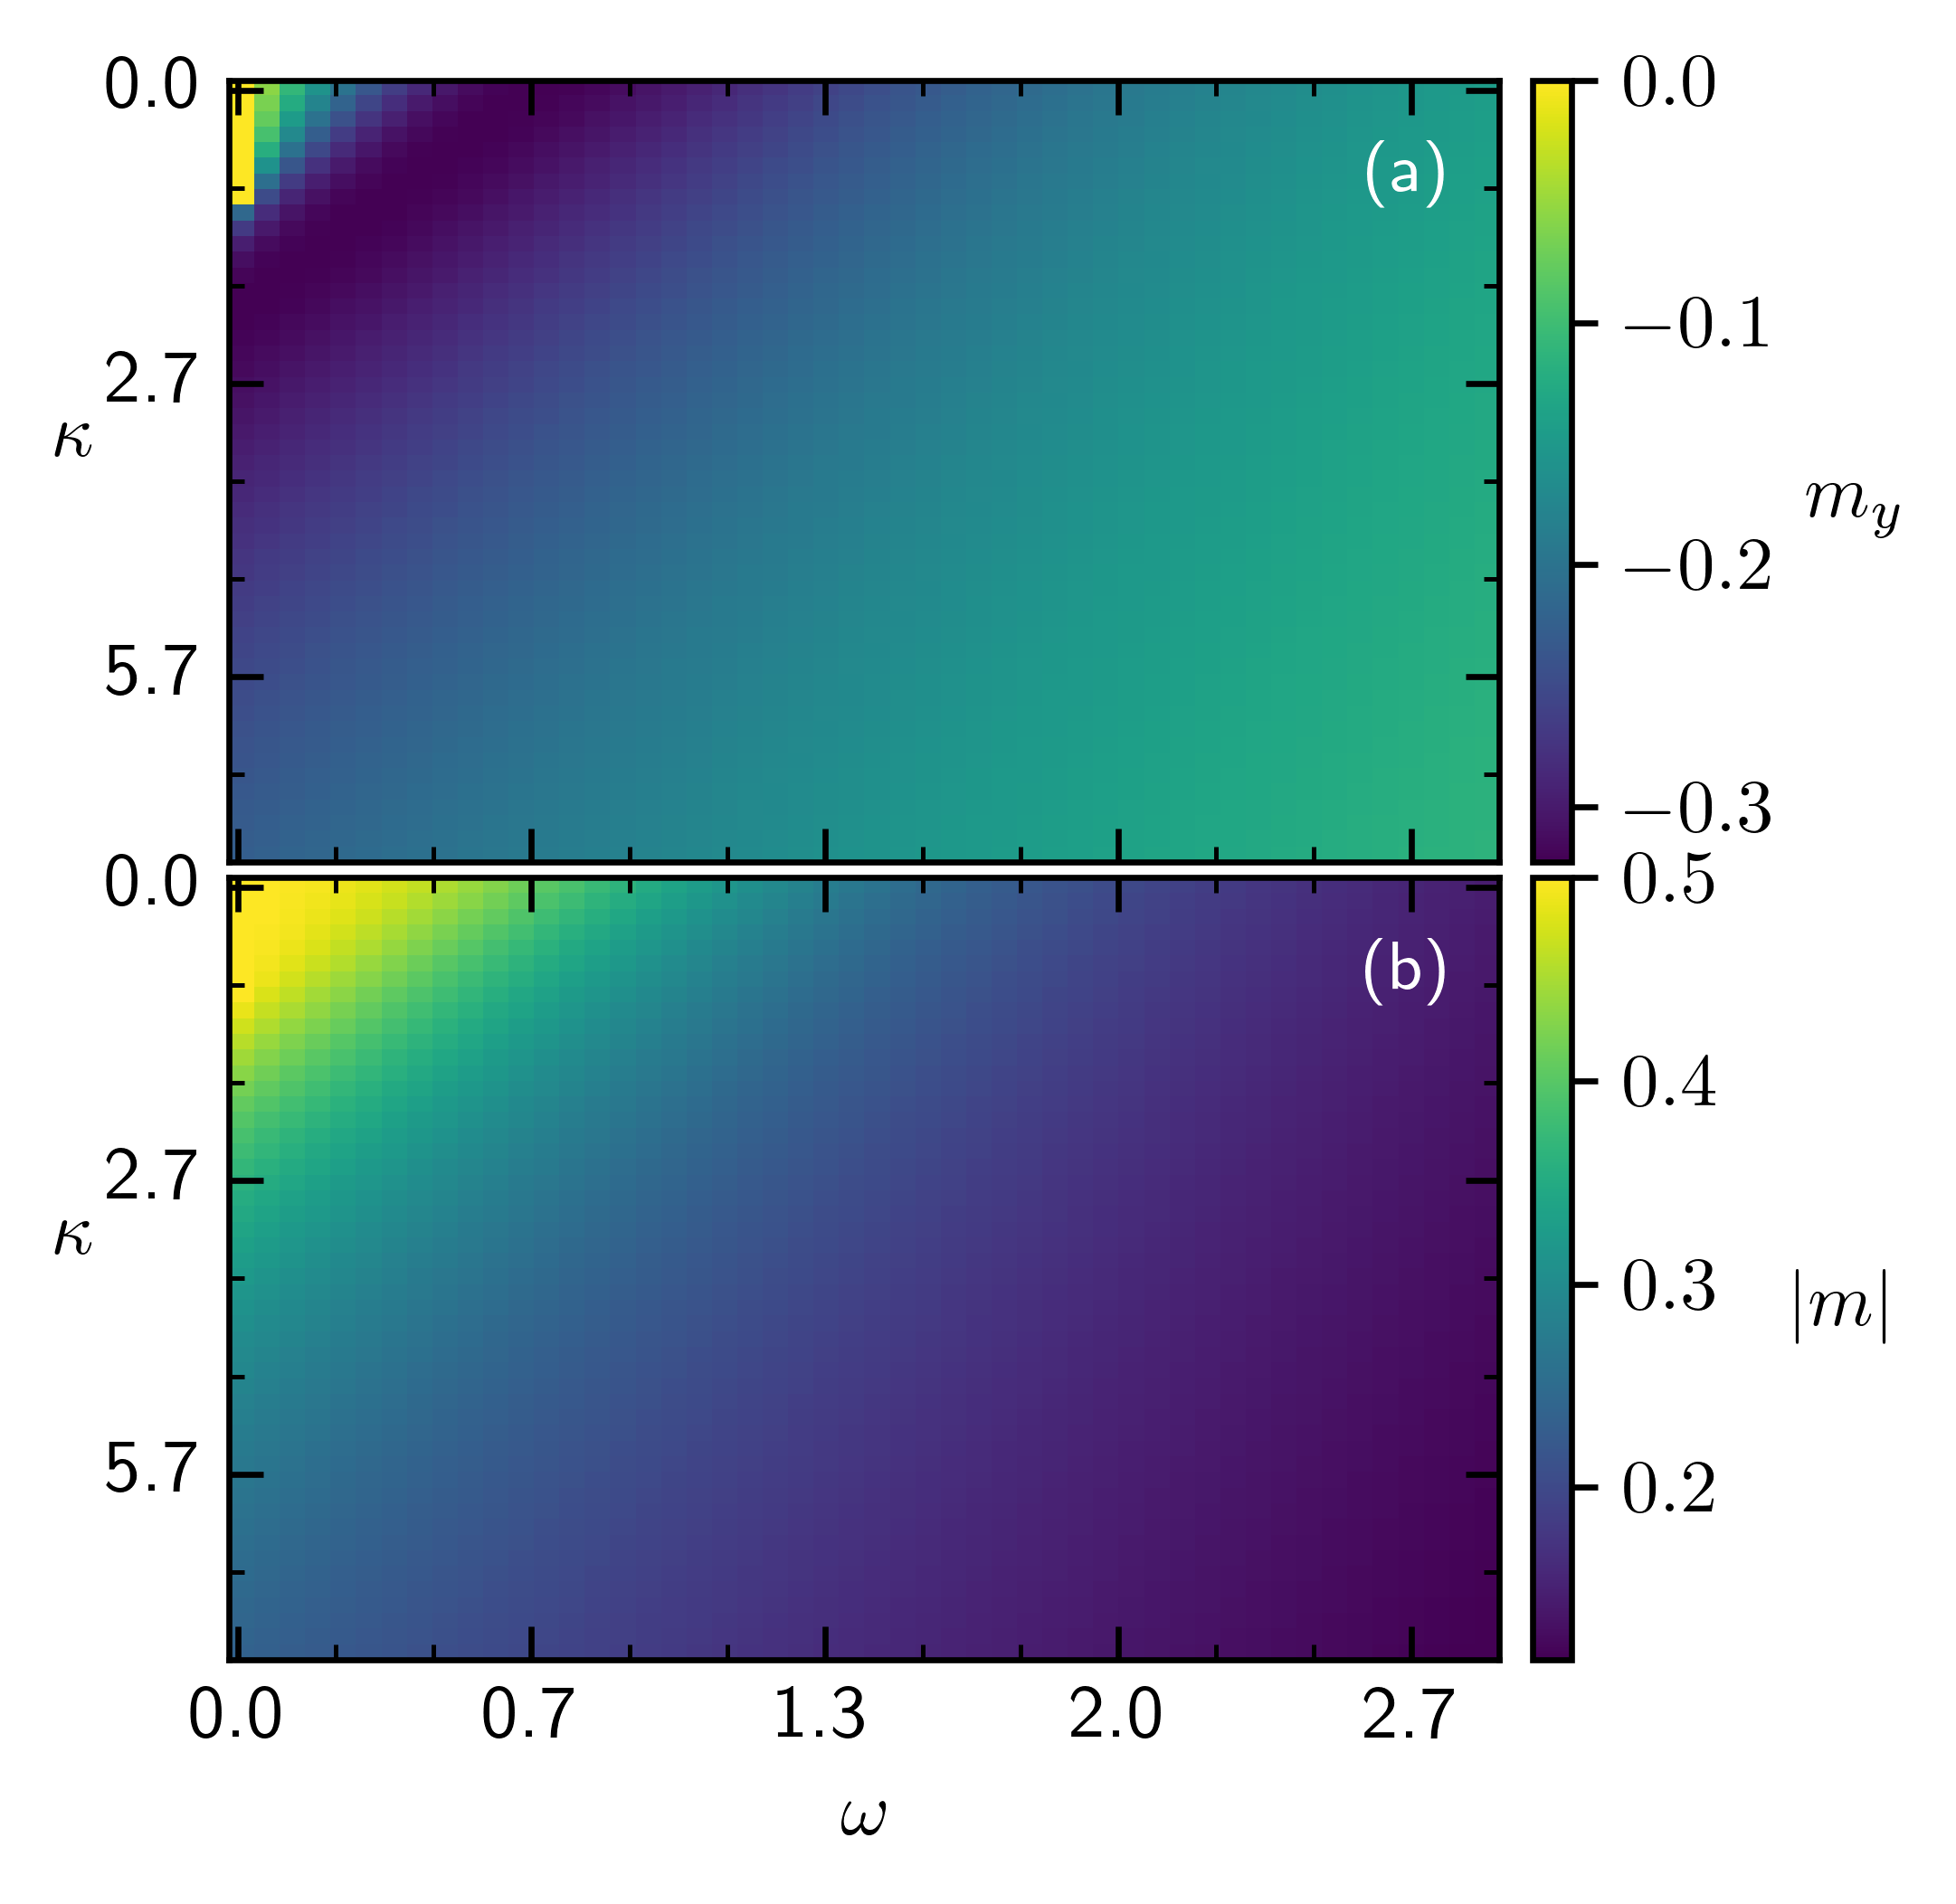
\includegraphics{pictures/fixp_bound_heatmap_s.png}
%     \vspace*{-2cm}\caption{Heatmap for the possible fixed point values for the small $m_y$-solution. (a) depicts $m_y$, whereas (b) depicts $|m|$-values.}
%     
% \end{wrapfigure}
\begin{figure}[H]
    % \floatbox[{\capbeside%\captionsetup[capbesidefigure]%{labelsep=newline}%
    % \thisfloatsetup{capbesideposition={right,center},capbesidewidth=none}}]{figure}[\FBwidth]
    \caption{Heatmap for the possible fixed point values for the small $m_y$-solution. (a) depicts $m_y$, whereas (b) depicts $|m|$-values.}
    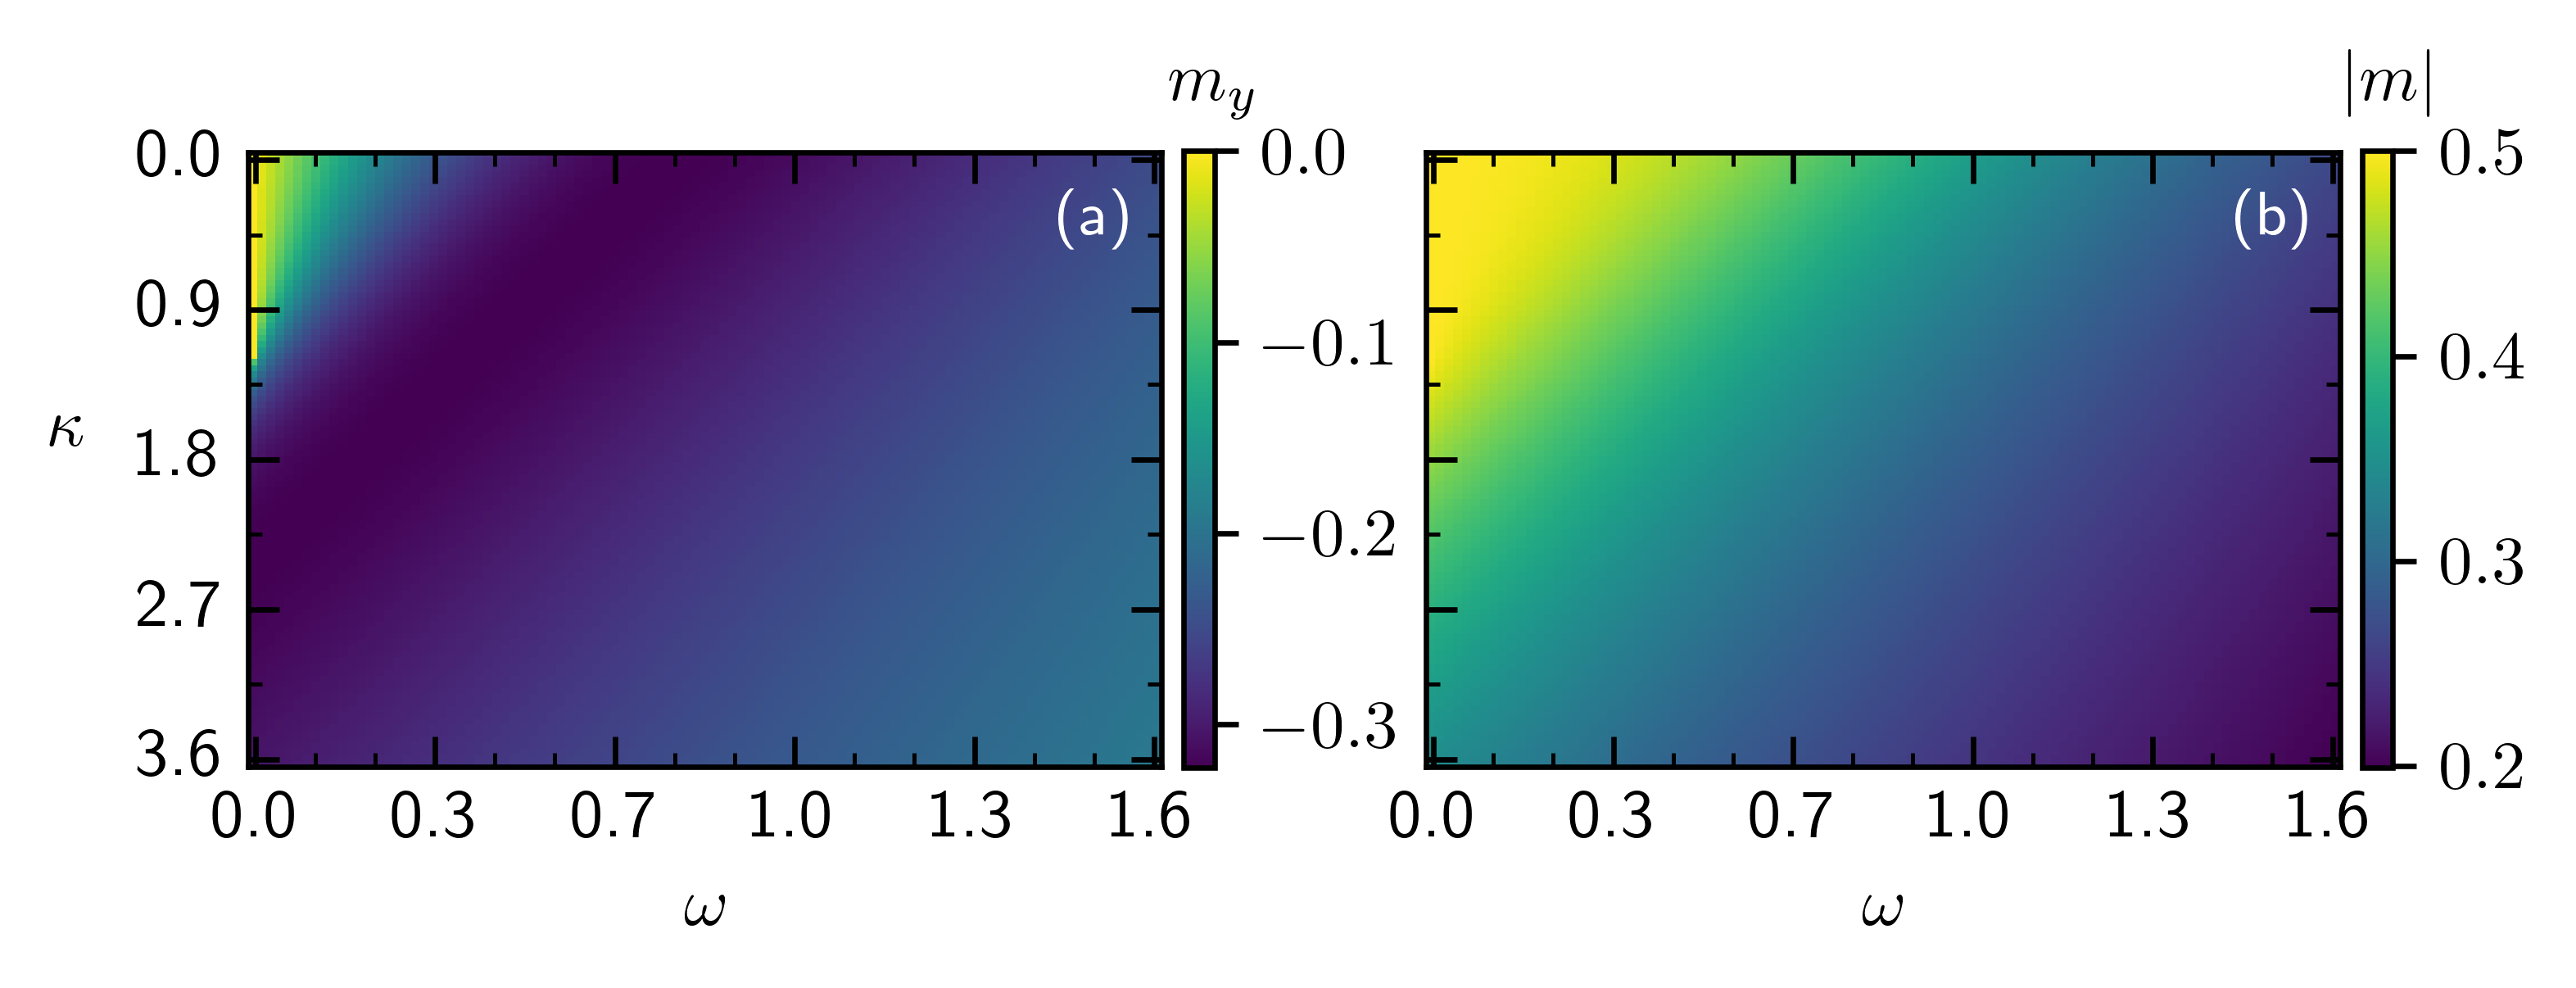
\includegraphics{pictures/fixp_bound_heatmap_s_horiz.png}
    \label{fig:fixp_small_bound_hm}
    %{\label{fig:num_of_fixp_criterium_BF}}
\end{figure}
\begin{figure}[H]
    \vspace*{-0.8cm}
    \hspace*{-1cm}
    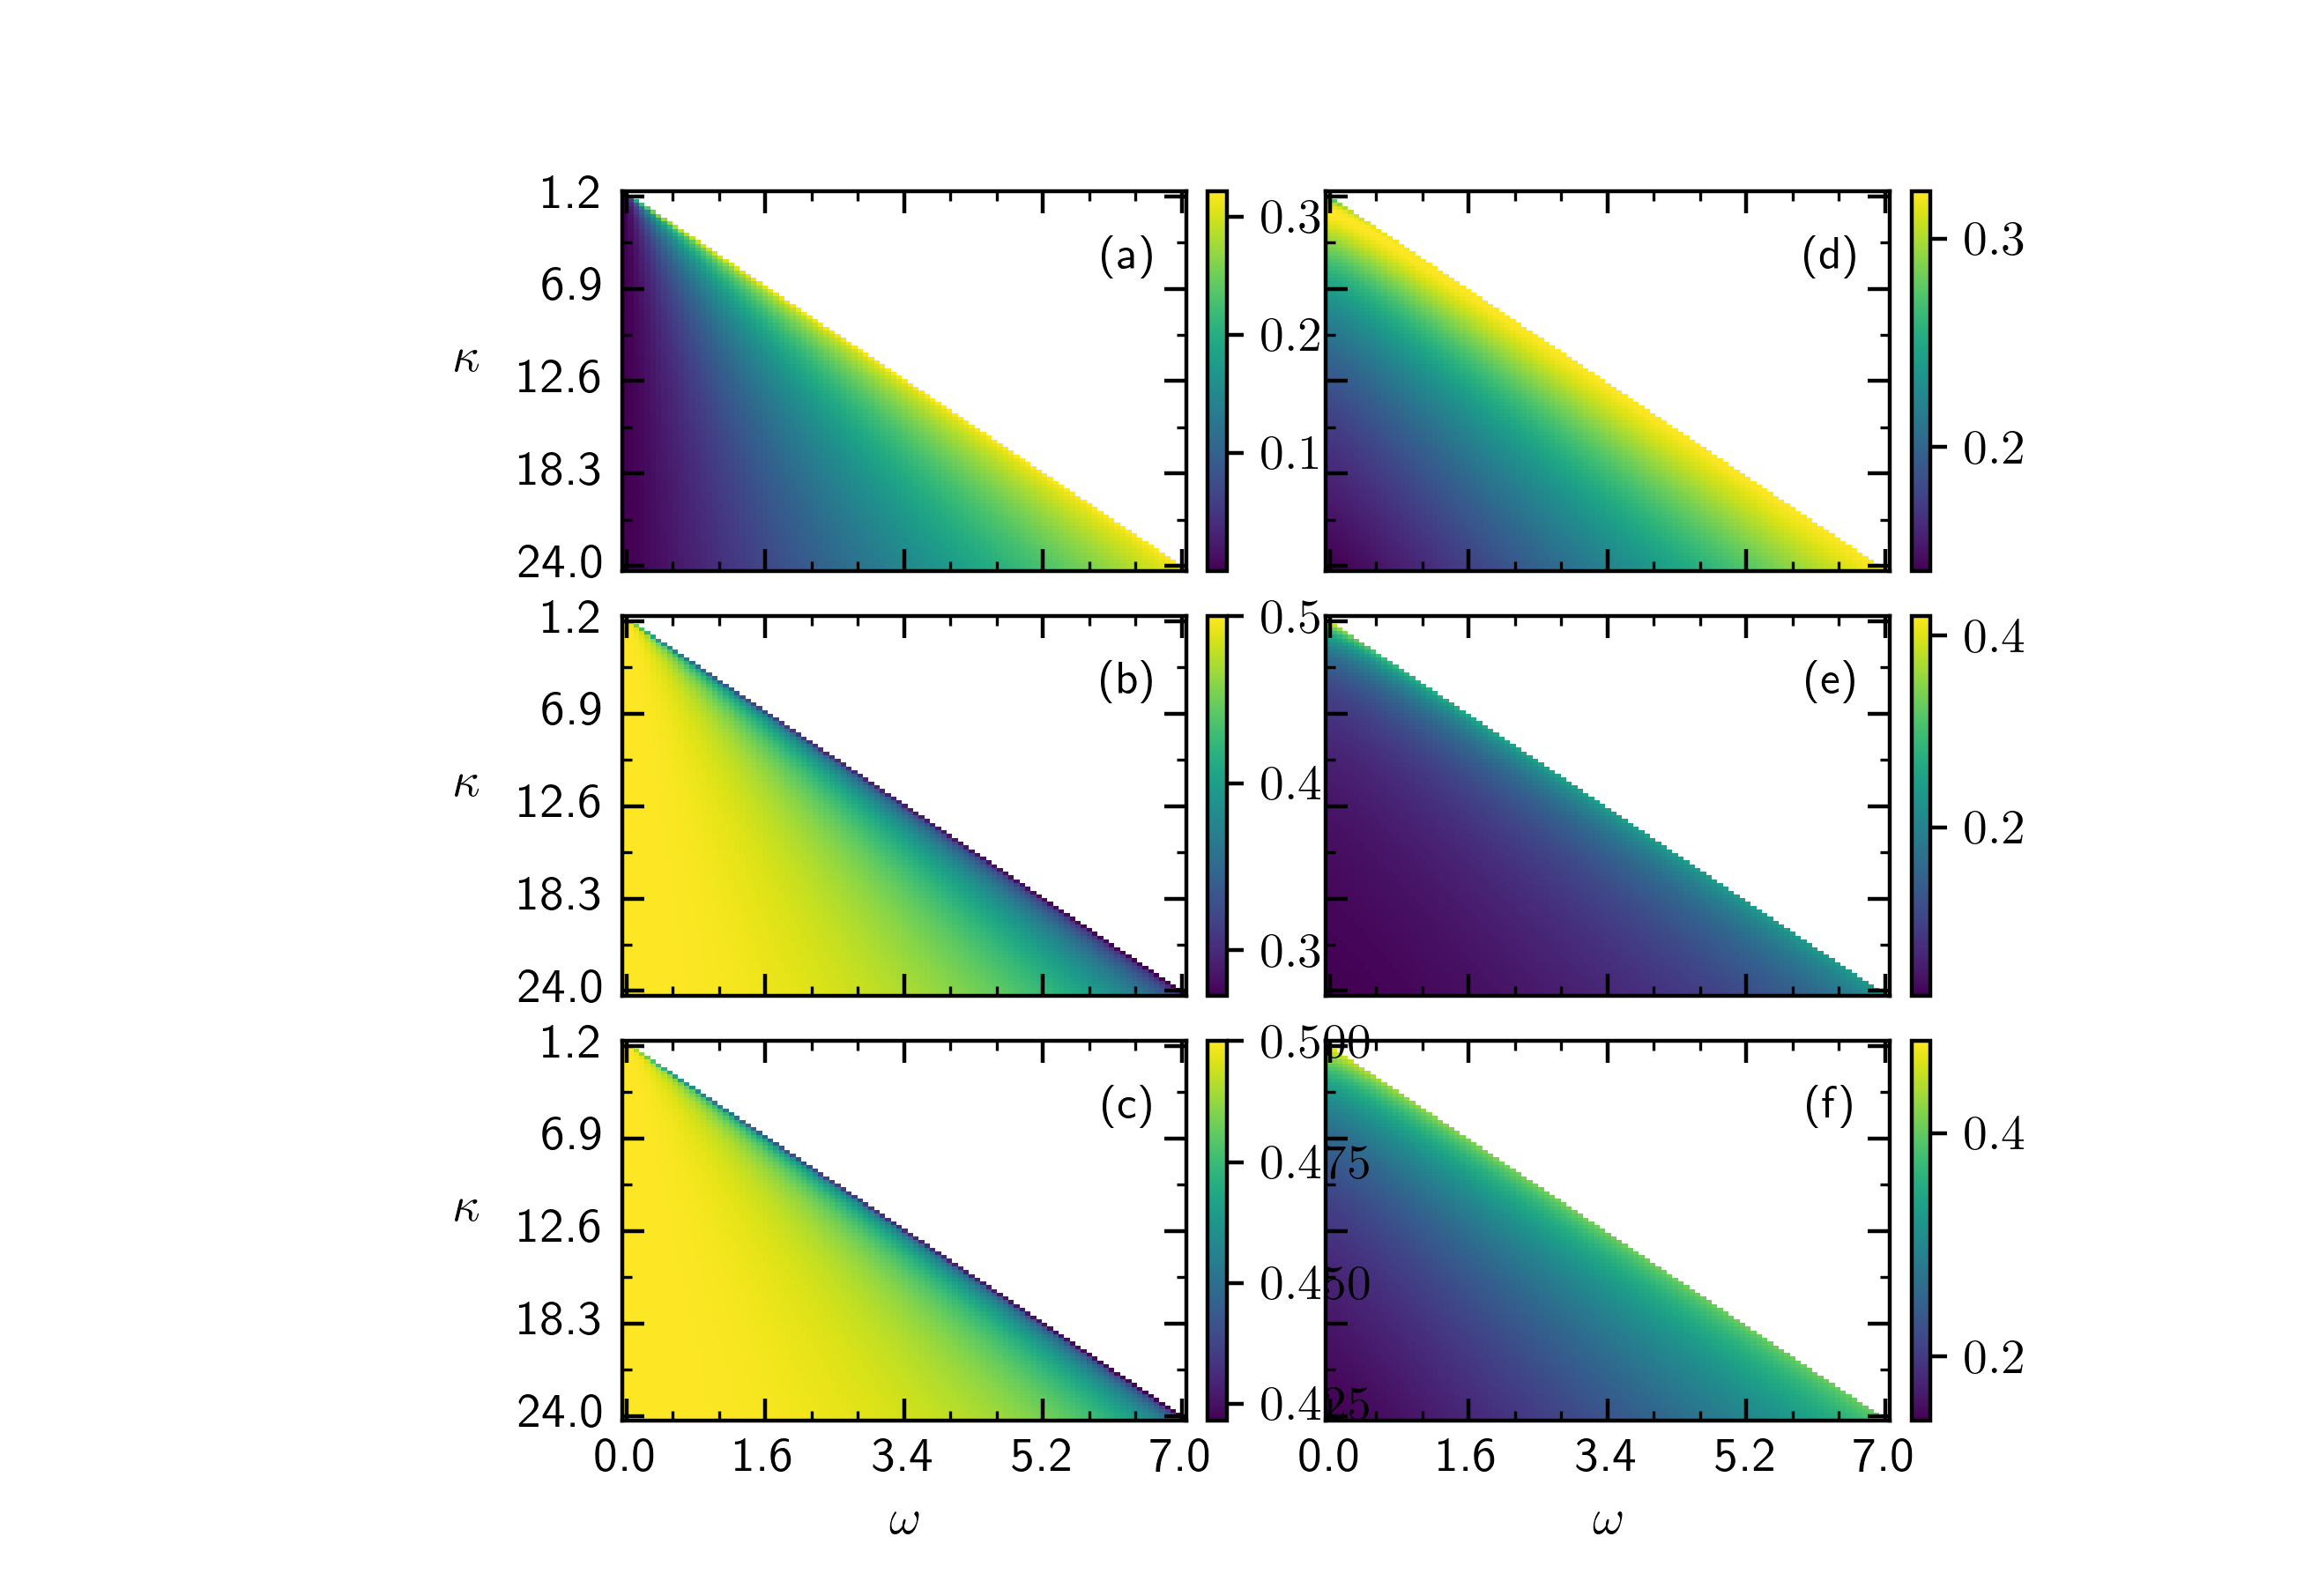
\includegraphics{pictures/fixp_bound_heatmap_ml2.png}
    \caption{heatmap of the range of the fixed point for a certain parameter range of $\omega$ and $\kappa$. $\Gamma=1$, $\gamma=0.2$ are fixed. Presented are properties of the middle $m_y$-solutions in diagrams (a-c) and for the larger $m_y$-solution in (d-f).}
    \label{fig:fixp_midlarge_bound_hm}
\end{figure}
For \figref{fig:fixp_small_bound_hm} and \figref{fig:fixp_midlarge_bound_hm} I calculated components of the collective spin as well as its modular value for different parameter configurations.
The column-like area of $m_y=0$ for small $\kappa$ and $\omega$ in \figref{fig:fixp_small_bound_hm}(a) stems from the fact that for $\omega=0$ and $A>0$ (i.e. $\kappa<\Gamma+\gamma$) $m_y=0$ is the constant solution to the stationary problem. For $A<0$ and $\omega=0$ the $y$-solution grows like $m_y\propto\sqrt{\kappa}$, whereas, for $A>0$ and constant, $m_y$ grows linearly with $\omega$ ($m_y\propto\omega$). Thus the somehow attention grabbing area in the top left corner of the $m_y$ plot can be explained by a constant part of the column at $\omega=0$ together with different grow regimes.
The fixed points are constraint to the physically allowed space, where $|m|\leq1/2$. In some cases the boundary is reached. Especially for the middle $m_y$ fixed point (\figref{fig:fixp_midlarge_bound_hm}(a-c)) $|m|$ is big for a wide range of parameters. Keep in mind that, as $m_z(m_y\rightarrow0)\rightarrow1/2$, the total collective spin reaches it's boundaries for small absolute values of $m_y$.\\\\
Summing up the findings of this paragraph, there are 2 different regions in parameter space. One area, where there exist 3 fixed points, is separated by a nearly linear border from a region of only one stationary solution.


\subsection{Stability analysis}
In order for stationary solutions to play a role in the long-time behavior of the system they need to be stable. This means there has to be at least a small area around the fixed point, so that the system, when starting from a point in this area, ends up in the fixed point for long times. If one makes the region of consideration around the fixed point small enough, the dynamics is governed by the linearization of the equations of motion with respect to $m$. In general one can consider the equation of motion for a function $\mathbf{x}=(x_1,x_2,x_3)^t$ that reads
\begin{align*}
    \dt \mathbf{x}=\mathbf{f}(\mathbf{x})=(f_1(\mathbf{x}),f_2(\mathbf{x}),f_3(\mathbf{x}))^t
\end{align*}
with any differentiable function $\mathbf{f}$. Up to first order in the difference between a point $\mathbf{x}$ and a stationary point of the equation of motion $\mathbf{x}^*$, the dynamics read 
\begin{align*}
    \dt \delta\mathbf{x} \vcentcolon&= \dt\,(\mathbf{x}-\mathbf{x}^*)=D\mathbf{f}|_{\mathbf{x}^*}\,\delta\mathbf{x}\\
    &=\vcentcolon\mathcal{C}\,\delta\mathbf{x}\quad,
\end{align*}
where $D\mathbf{f}|_{\mathbf{x}^*}$ is the Jacobian of $\mathbf{f}$. The emerged linear differential equation is solved by a simple matrix exponential
\begin{align*}
    \delta\mathbf{x}(t)=\delta\mathbf{x}(t=0)\,\exp(\mathcal{C}t)
\end{align*}
For a diagonalizable matrix $\mathcal{C}$, $\delta\mathbf{x}$ can be represented in an eigenbasis of $\mathcal{C}$. The component related to a member of the eigenbasis grows or decays exponentially with the according eigenvalue as rate. For a matrix with all negative eigenvalues a small deviation from the stationary point returns back to it, making this fixed point stable. \\If at least one eigenvalue is positive, the region around the stationary point contains an at least one dimensional subspace, for which points lying on this subspace depart from the fixed point with growing time. \\In this scenario, for an implementation of our model to a real physical system, the presence of unavoidable fluctuations would push the collective spin slightly away from the stable subspace, from where it would exponentially depart from the fixed point\cite{pikovskij_synchronization_2007}. Hence fixed points that are not fully stable will not behave as attractors for the collective spin, even in their vicinity. For the case of an eigenvalue getting zero, one has to turn to the next order for an evaluation of the stability.\\\\
% \begin{figure}[H]
%     \hspace*{-1cm}
%     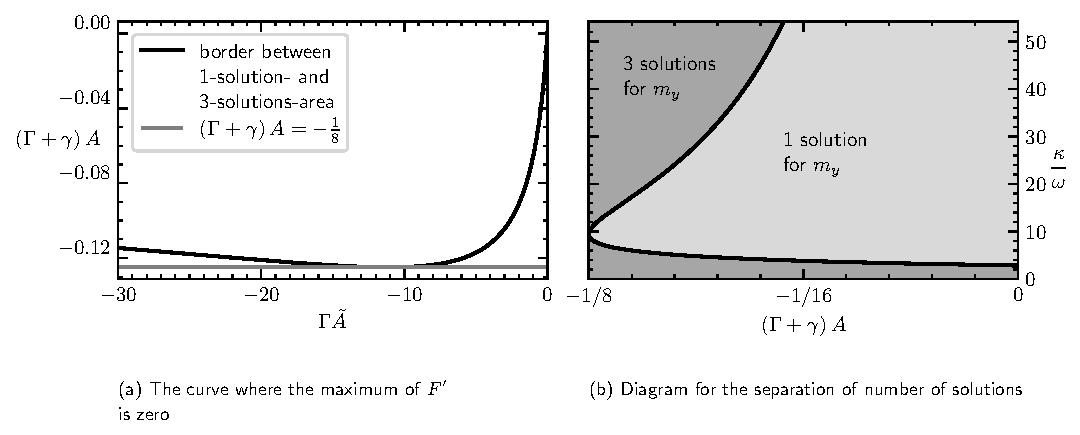
\includegraphics{pictures/phaseplot_A_kw.pdf}
%     \caption{The parameter configurations, where there are 1 ore 3 fixed points can be separated.}
%     \label{fig:phases_numb_of_fixp}
% \end{figure}
With this information in mind one can now move on to the analysis of the stability of the previously found stationary points, knowing that only points, where the linearization matrix has all negative eigenvalues, qualify as certain attractors. The starting of the examination is the calculation of the linear expansion of the equations of motion.
\begin{align*}
    \dt\left(\begin{array}{c}
         \delta m_x\\
         \delta m_y\\
         \delta m_z
    \end{array}\right)&=\left( \begin{array}{ccc}
        -\Gamma\,A-y^2+\frac{\tilde{\omega}}{\tilde{\kappa}}\,y&  0 & 0\\
        0 & -\Gamma\,A-y^2+\frac{\tilde{\omega}}{\tilde{\kappa}}\,y & \sqrt{2}\,\frac{\Gamma}{\tilde{\kappa}^2}\,(\tilde{\kappa}\,y-\tilde{\omega})\\
        0 &  -\sqrt{2}\,\frac{\Gamma}{\tilde{\kappa}^2}\,(2\tilde{\kappa}\,y-\tilde{\omega}) & -2\,\frac{\Gamma^2}{\tilde{\kappa}^2}
    \end{array} \right)\,\left(\begin{array}{c}
         \delta m_x\\
         \delta m_y\\
         \delta m_z
    \end{array}\right)
\end{align*}
For the analysis of the sign of the eigenvalues one is free to multiply the matrix with a positive number, i.e $\tilde{\kappa}^2/\tilde{\omega}^2$, what yields the matrix
\begin{align*}
    \mathcal{C}=\left( \begin{array}{ccc}
        -\Gamma A-{y}^2+{y}&  0 & 0\\
        0 & -\Gamma A-{y}^2+{y}& \sqrt{2}\,\Gamma/\tilde{\kappa}\,({y}-\frac{\tilde{\kappa}}{\tilde{\omega}})\\
        0 &  -\sqrt{2}\,\Gamma/\tilde{\kappa}\,(2\,{y}-\frac{\tilde{\kappa}}{\tilde{\omega}}) & -2\,\frac{\Gamma^2}{\tilde{\omega}^2}
    \end{array} \right)
\end{align*}
The first eigenvalue is already accessible due to the block form of the matrix. In order to determine the sign of the first eigenvalue in general, it is convenient to define an even more general parameter
% \begin{wrapfigure}[16]{l}{0pt}
\begin{figure}[H]
    \centering
    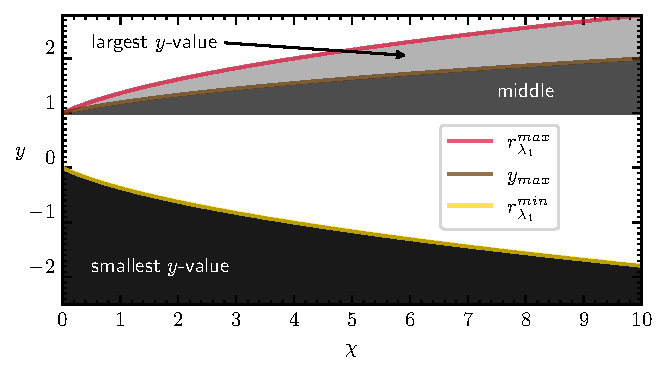
\includegraphics{pictures/sign_of_ev1_streched.pdf}
    % \vspace*{-2cm}
    \caption{The smaller ($r_{\lambda_1}^{min}$) and larger ($r_{\lambda_1}^{max}$) roots of $\lambda_1$ with marked areas for the value for ${y}=k/w\cdot m_y$. ${y}_{max}$ is the ${y}$-position of $F$.}
    \label{fig:sign_lam1}
\end{figure}
% \end{wrapfigure}
\begin{gather*}
    \chi\vcentcolon=\frac{K-1}{\Omega^2}\\
    \Rightarrow\quad\Gamma A=-\half\,\chi,\quad
    B=\half\,\chi+\frac{1}{2\,\Omega^2}%\frac{K}{2\,\Omega^2}&=\frac{K-1}{2\,\Omega^2}+\frac{1}{2\,\Omega^2}=\half\,\chi+\frac{1}{2\,\Omega^2}
\end{gather*}
The first eigenvalue is in the form of a second order polynomial in $y$ and has therefore in general 2 roots. Between the two roots the eigenvalue is positive marking the fixed point as unstable, where as outside the interval between the roots the eigenvalue is negative, maintaining the possibility of a stable fixed point. When the parameter $\chi$ gets negative \figref{fig:sign_lam1} shows, that the roots of $\lambda_1$ lie both in the region $y>0$. From the previous consideration it is known, that only one fixed point exists for $\chi<0$, i.e $K<1$, and it is negative. Thus for $\chi<0$ the first eigenvalue is always negative.\\\\
Turning to the case $K>1$. Here 3 fixed points are possible. Picturing a possible course of the polynomial of third degree, whose solutions resemble the $y$-values of the fixed points one can make a few statements on the position of those fixed points. The smallest solution, which is always negative, has its maximal value for the shift $B$ being minimal. For a given parameter configuration, it always holds $B<\chi/2$. So the values of the smallest solution, if $B$ is replaced by $\chi$ are always larger as the true solution. In fact $B\rightarrow\chi$ when $\Omega\rightarrow\infty$ and also $K$ diverges in a way that keeps $\chi$ constant.
\begin{align*}
    \tilde{F}({y})=-\half\,\chi-(1-\half\,\chi)\,{y}    - {y}^3+2\,{y}^2
\end{align*}
% For a given value of $\chi$ the parameter $\Omega$ can be chosen freely, because through an appropriate choice of $K$ the value of $\chi$ can be fixed. So for every possible value of $\chi>0$ the supreme value of $B$ is just $\chi/2$, as $\Omega\rightarrow\infty$.
% The first, smallest fixed point has again because of the positive sign of $B$ always a negative $y$-component. It has it's greatest value for minimal $B$. Negative values of $\chi$ lead to positive roots of $\lambda_1$, which induces that $\lambda_1$ itself is negative. \\\\
It turns out that the roots of $\lambda_1$ are always a root of $\tilde{F}$. Consequently the true $y$-value of the fixed point, with smallest $y$, is always smaller than the root of $\lambda_1$ and therefore this fixed point has a negative first eigenvalue.\\\\
So I will move on to the next fixed point, the one in the middle. It also takes its smallest value for minimal $B$, allowing one to look at the function $\tilde{F}$ again. In this constellation the middle root is always at ${y}=1$. The maximal possible $y$-value (actually supremum) for the middle fixed point is at the maximum point of $F$ which is also the minimal possible value of the largest root. The maximum $y$-value of the largest fixed point, is again for minimal $B$ and thus the larger root of $\lambda_1$ is a supremum of this fixed point.\\\\
In summary one can state that the first eigenvalue of the smallest-$y$ solution is always negative, whereas the eigenvalue of the other possible fixed points is always positive, identifying them as unstable. \\\\As unstable fixed points are from a physical perspective not as significant, I will focus in the following part of the discussion mainly on the fixed point with smallest $y$-solution. The stability of this stationary solution is yet to be determined by evaluating the remaining eigenvalues.
% $K$ and $\Omega$ can always be adopted in a way, so that $\chi$ and $1/\Omega^2$ can take every arbitrarily large number.
% \begin{gather*}
%     \frac{K-1}{\Omega^2}=\chi, \quad \frac{1}{\Omega^2}=M\\
%     \Rightarrow K=1+\frac{\chi}{M}\quad\text{and}\quad\Omega = \frac{1}{\sqrt{M}}
% \end{gather*}
% Thus the true $B$ can be made arbitrarily big while $\chi$ stays as it is, allowing in turn, that the fixed point, with the largest $y$-value, gets arbitrarily large.
% So we can already provide a diagramm for the possible sign-values of $\lambda_1$ in \autoref{fig:sign_lam1}.\\\\
This analysis will be performed numerically. Thus there is less need for rescaling quantities, instead it is often more convenient to stick to the original form, in order to avoid unnecessary pols. In this form $m_y$ is determined by the equation
\begin{align*}
    0=&-\half\,\Gamma\omega-(\half\,\Gamma\,(\Gamma+\gamma-\kappa)+\omega^2)\,m_y\\&-\kappa^2\,m_y^3+2\,\kappa\omega\,m_y^2
\end{align*}
and the linearization of the equations of motion result in the following matrix.
\begin{align*}
    \Gamma\,\mathcal{C}=&\left( \begin{array}{c c c}
        -\half\,\Gamma\,(\Gamma+\gamma-\kappa)-\kappa^2\,m_y^2
        +\omega\kappa\,m_y&0&0\\
        0&-\half\,\Gamma\,(\Gamma+\gamma-\kappa)-\kappa^2\,m_y^2
        +\omega\kappa\,m_y&\Gamma\,(\kappa\,m_y-\omega)\\
        0&-\Gamma\,(2\kappa\,m_y-\omega)&-\Gamma^2
    \end{array}  \right)
\end{align*}

% \begin{wrapfigure}[29]{l}{0pt}
%     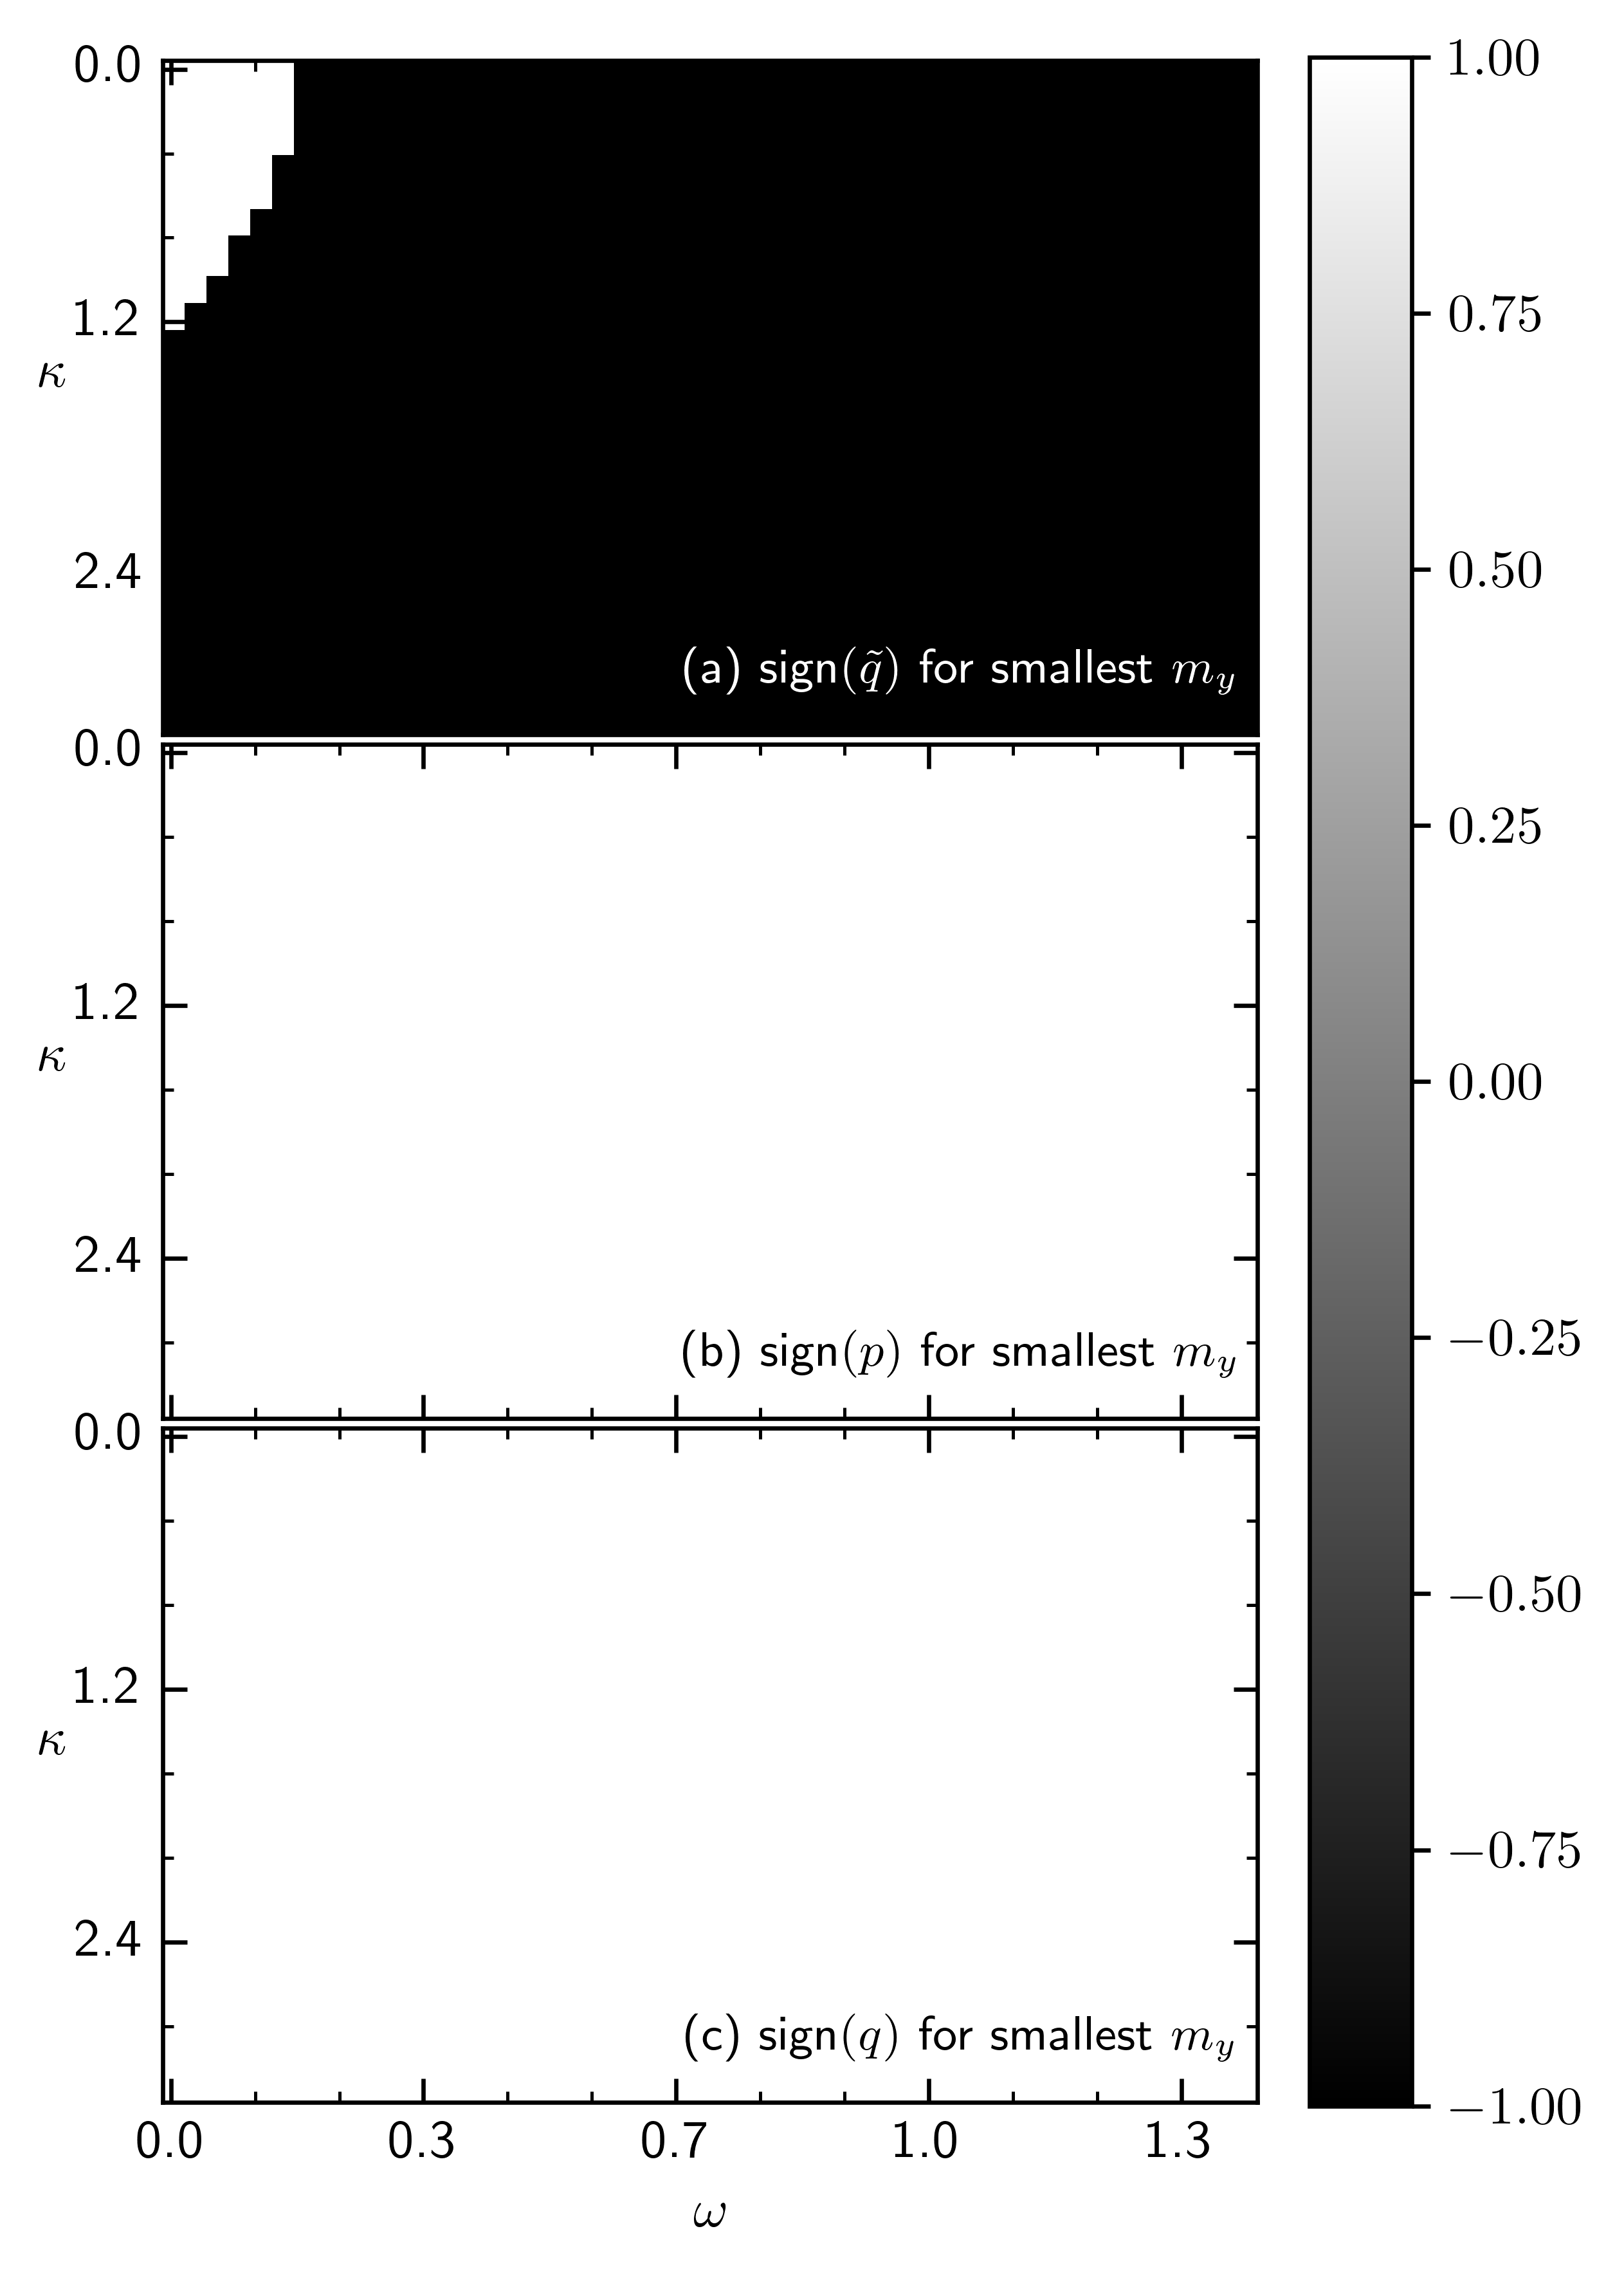
\includegraphics{pictures/lam2_anal_s.png}
%     \vspace*{-2cm}\caption{Heatmap for the possible fixed point values for the small $m_y$-solution. (a) depicts $m_y$, whereas (b) depicts $|m|$-values.}
%     \label{fig:sign_lam23_s}
% \end{wrapfigure}


The remaining two eigenvalues of the fixed points are the eigenvalue of the lower $2\times2$-block of the linearization matrix and are determined by the $\lambda$-roots of the expression
\begin{align*}
    0&=\lambda^2+\left( \Gamma^2 +\half\,\Gamma\,(\Gamma+\gamma-\kappa)+\kappa^2\,m_y^2
    -\omega\kappa\,m_y\right)\,\lambda\\
    &+\Gamma^2\,(\half\,\Gamma\,(\Gamma+\gamma-\kappa)+\kappa^2\,m_y^2-\omega\kappa\,m_y)\\
    &+\Gamma^2\,(\kappa\,m_y-\omega)\,(2\,\kappa\,m_y-\omega)\\
    &=\vcentcolon t^2+p\,t+q\\
    \Rightarrow\quad\lambda_{23}&=\half\,(-p\pm\sqrt{p^2-4q})\quad.
\end{align*}
% or
% \begin{align*}
%     0=&\,t^2+\left( 2\,\frac{\Gamma^2}{\tilde{\omega}^2}+\Gamma\tilde{A}+y^2-y \right)\,t\\
%     &+2\,\frac{\Gamma^2}{\tilde{\omega}^2}\,\left( \Gamma\tilde{A}+y^2-y \right)\\
%     &+2\,\frac{\Gamma^2}{\tilde{\kappa}^2}\,(2\,y-\frac{\tilde{\kappa}}{\tilde{\omega}})\,(y-\frac{\tilde{\kappa}}{\tilde{\omega}})\\
%     &=\vcentcolon t^2+p\,t+q\\
%     \Rightarrow\quad\lambda_{23}=&\half\,(-p\pm\sqrt{p^2-4q})\quad.
% \end{align*}
When $q$ becomes negative, the square root gets larger in absolute value than $p$ and thus one eigenvalue is positive, resulting in an unstable fixed point. On the other hand, when $p$ and $q$ are both positive, both eigenvalues $\lambda_{23}$ have negative real part.

\begin{figure}[H]
    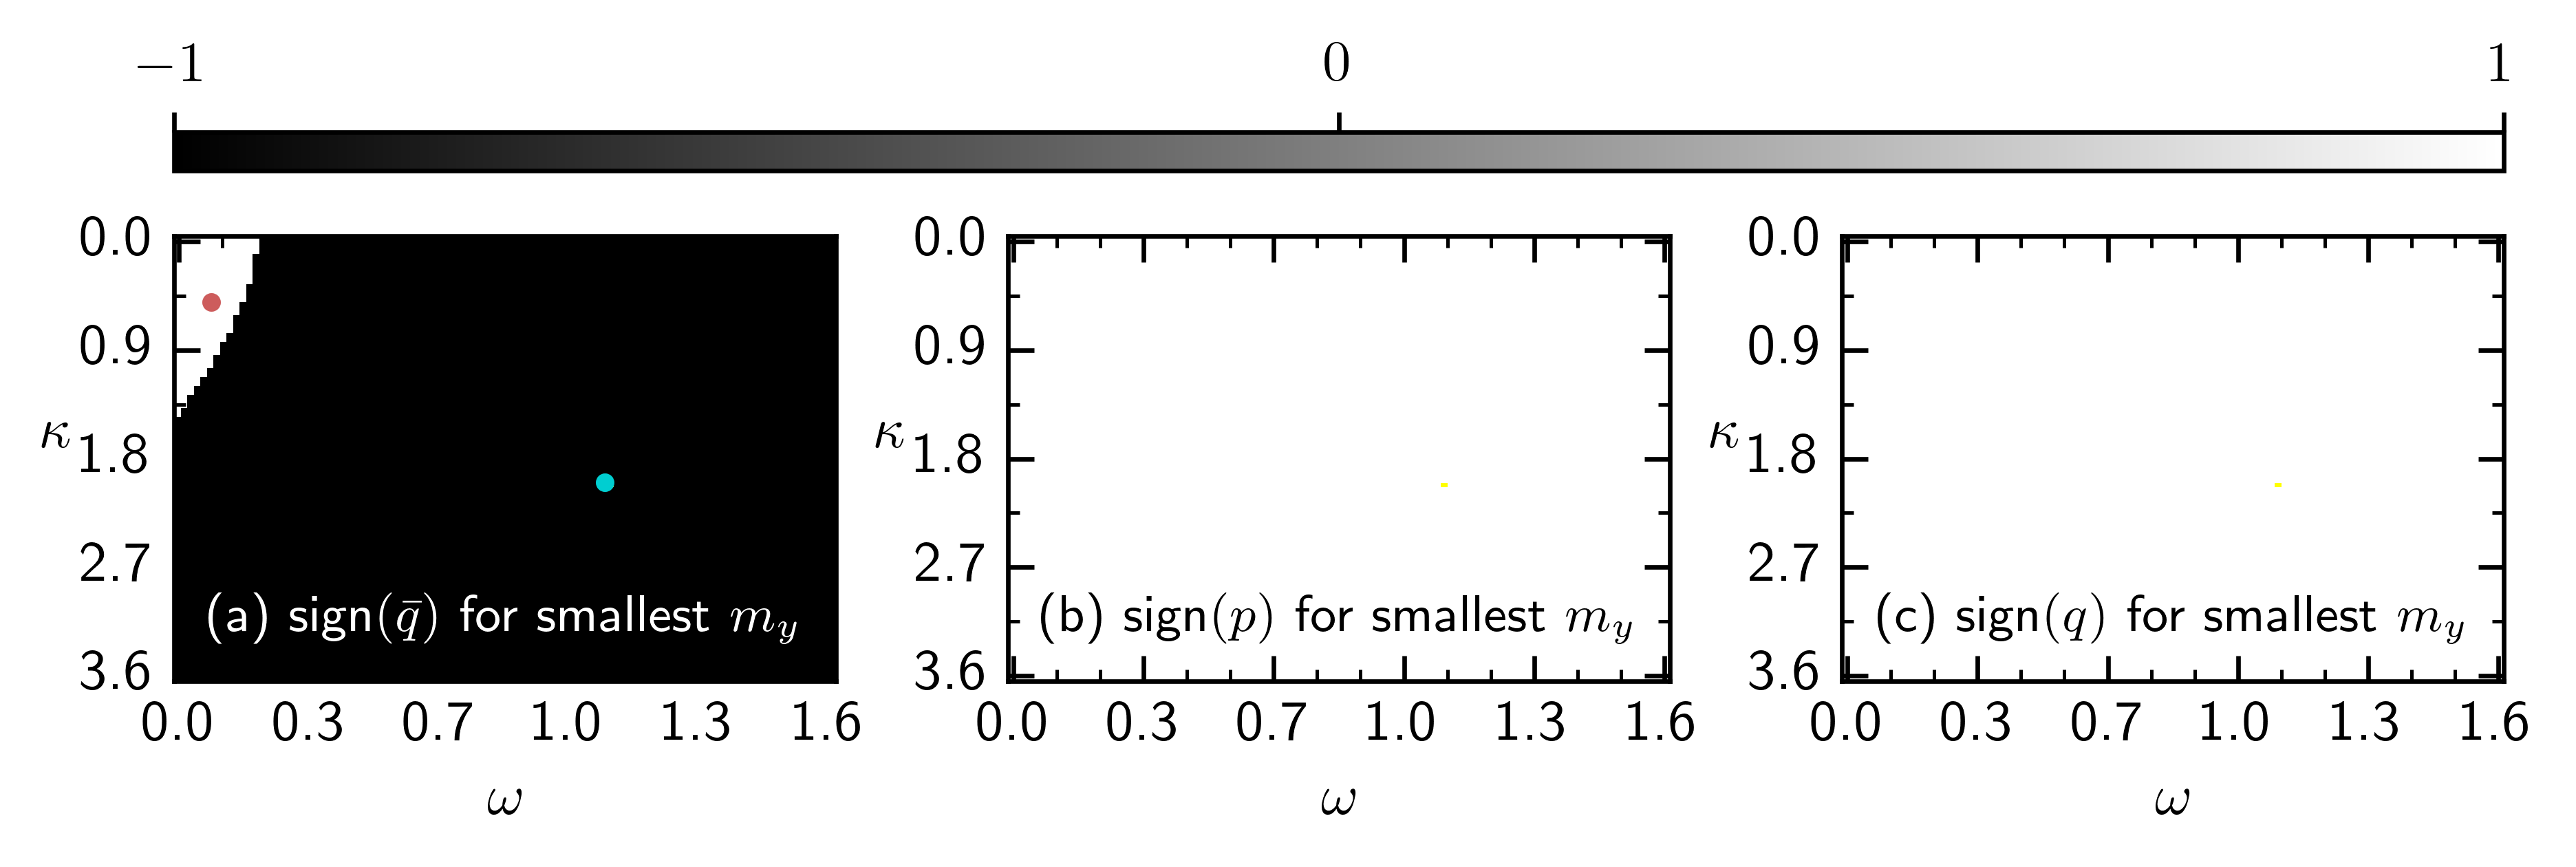
\includegraphics{pictures/lam2_anal_s2.png}
    \caption{Sign analysis of eigenvalue 2 and 3 for the smallest $y$-valued stationary point. In (a) the sign of the interior of the square root, involved in the formula for these eigenvalues, is shown and hence complex eigenvalues are indicated. For the red and blue dots exemplary trajectories are plotted below, confirming the presence or absence of oscillatory behavior. (b) and (c) show that the sign of the quantities $p$ and $q$.}% are both always positive, and thus the whole eigenvalue has negative real part.}
    \label{fig:sign_lam23_s}
\end{figure}%
As can be observed from \figref{fig:sign_lam23_s} (b)-(c) $p$ and $q$ are always positive for the fixed point with smallest $y$-value and hence this stationary point is stable for all considered parameter configurations.\\
From the information, whether the eigenvalues are real or complex, a hint about the type of the dynamics can be derived. In the case of complex eigenvalues, which arise, if the discriminant of the characteristic polynomial $\bar{q}\vcentcolon=p^2-4q$ gets negative,  the matrix exponential has an oscillatory part. This is expected to also show in the full dynamics, if the system is sufficiently close to such a stationary point. To confirm this I took one parameter configuration in each of the two regions, where the eigenvalues become complex versus where they stay real. Their location is shown in \figref{fig:sign_lam23_s} (a). For those parameter configurations I calculated four exemplary trajectories starting at random points in the spin space, which are depicted in \figref{fig:expl_traj_d0}.
% Starting with the analysis of $p$ and going back one last time in the rescaled form with the above defined new parameters, one finds
% \begin{align*}
%     p=&\frac{\Gamma}{\Omega^2\,(\Gamma+\gamma)}-\half\,\chi+3\,y^2-4\,y+1
% \end{align*}
% the roots of this expression, which are maximally apart from each other, are found, when $\Omega\rightarrow\infty$ in the same spirit as above. This yields as roots of $p$
% \begin{align*}
%     r_p=&\frac{1}{3}\,\left( 2\pm\sqrt{1+\frac{3}{2}\,\chi-3\,\frac{\Gamma}{\Omega^2\,(\Gamma+\gamma)}} \right)\\
%     r_p^\text{max}=&\frac{1}{3}\,\left( 2+\sqrt{1+\frac{3}{2}\,\chi} \right)\\
%     r_p^\text{min}=&\frac{1}{3}\,\left( 2-\sqrt{1+\frac{3}{2}\,\chi} \right)
% \end{align*}
% One can recognize, that $r_p^\text{max}=\tilde{y}_\text{max}$ and $r_p^\text{min}=\tilde{y}_\text{min}$. Thus we can infer that for the bracketing fixed points $p$ is always positive, whereas for the middle fixed point we can't make this statement. Together with the finding that $q$ is positive this induces that the fixed point with smallest $y$-value is stable.\\\\
% For the unstable fixed points the analysis of the eigenvalues $\lambda_{23}$ is done numerically by the computing the expression
% \begin{align*}
%     \lambda_{23}=&\half\,(-p\pm\sqrt{p^2-4q})\quad.
% \end{align*}
% When $q$ becomes negative, the square roots gets larger in absolute value than $p$ and thus one eigenvalue is positive, resulting in an unstable fixed point. On the other hand, when $p$ and $q$ are both positive, both eigenvalues $\lambda_{23}$ have negative real part. The eigenvalues become complex and allow for oscillatory behavior near the fixed point if the interior of the square root, labeled as  
% \begin{align*}
%     \bar{q}\vcentcolon=p^2-4q\quad.
% \end{align*}
% get's negative. To describe the properties of the fixed points we investigate the three values $p$, $q$ and $\bar{q}$. %As already mentioned a negative $\bar{q}$ signals complex eigenvalues. In this case $-p$ is the real part of the eigenvalue. On the other hand when $q$ gets negative the eigenvalues $\lambda_2$ and $\lambda_3$ have different signs, whereas when $q\geq0$ the eigenvalues $\lambda_{23}$ have always the oposite sign of $p$
\begin{figure}[H]
    \centering
    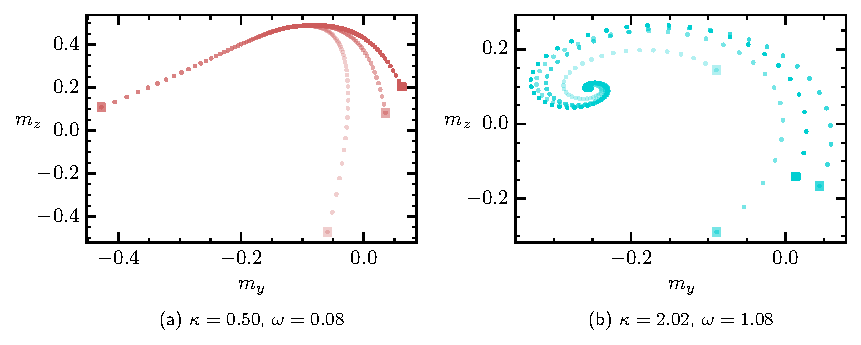
\includegraphics{pictures/example_traj_d0.pdf}
    \caption{For the two different parameter constellations in the area of complex (b) and all real (a) eigenvalues four trajectories are plotted starting at randomly chosen starting points. The starting points are marked by squares. In the two figures the different level of opacity is used to differentiate the trajectories.
    }
    \label{fig:expl_traj_d0}
\end{figure}

The evaluated trajectories show the expected behavior. Whereas for the case of all real eigenvalues the collective spin decays in a straight forward fashion to its stationary point, for complex eigenvalues the origin of oscillatory behavior arises. %Nevertheless for the case of $\delta=0$ these oscillations are damped, bringing the system for long times to a constant stationary point.
\\\\An indication to the speed of this decay is given by the magnitude of the eigenvalues, which are plotted in \figref{fig:eig_value_stab1} and \figref{fig:eig_value_stab2}. The less significant values of the unstable fixed points are shown in \appref{appendix:eig_del0} for completeness.

\begin{figure}[H]
    \centering
    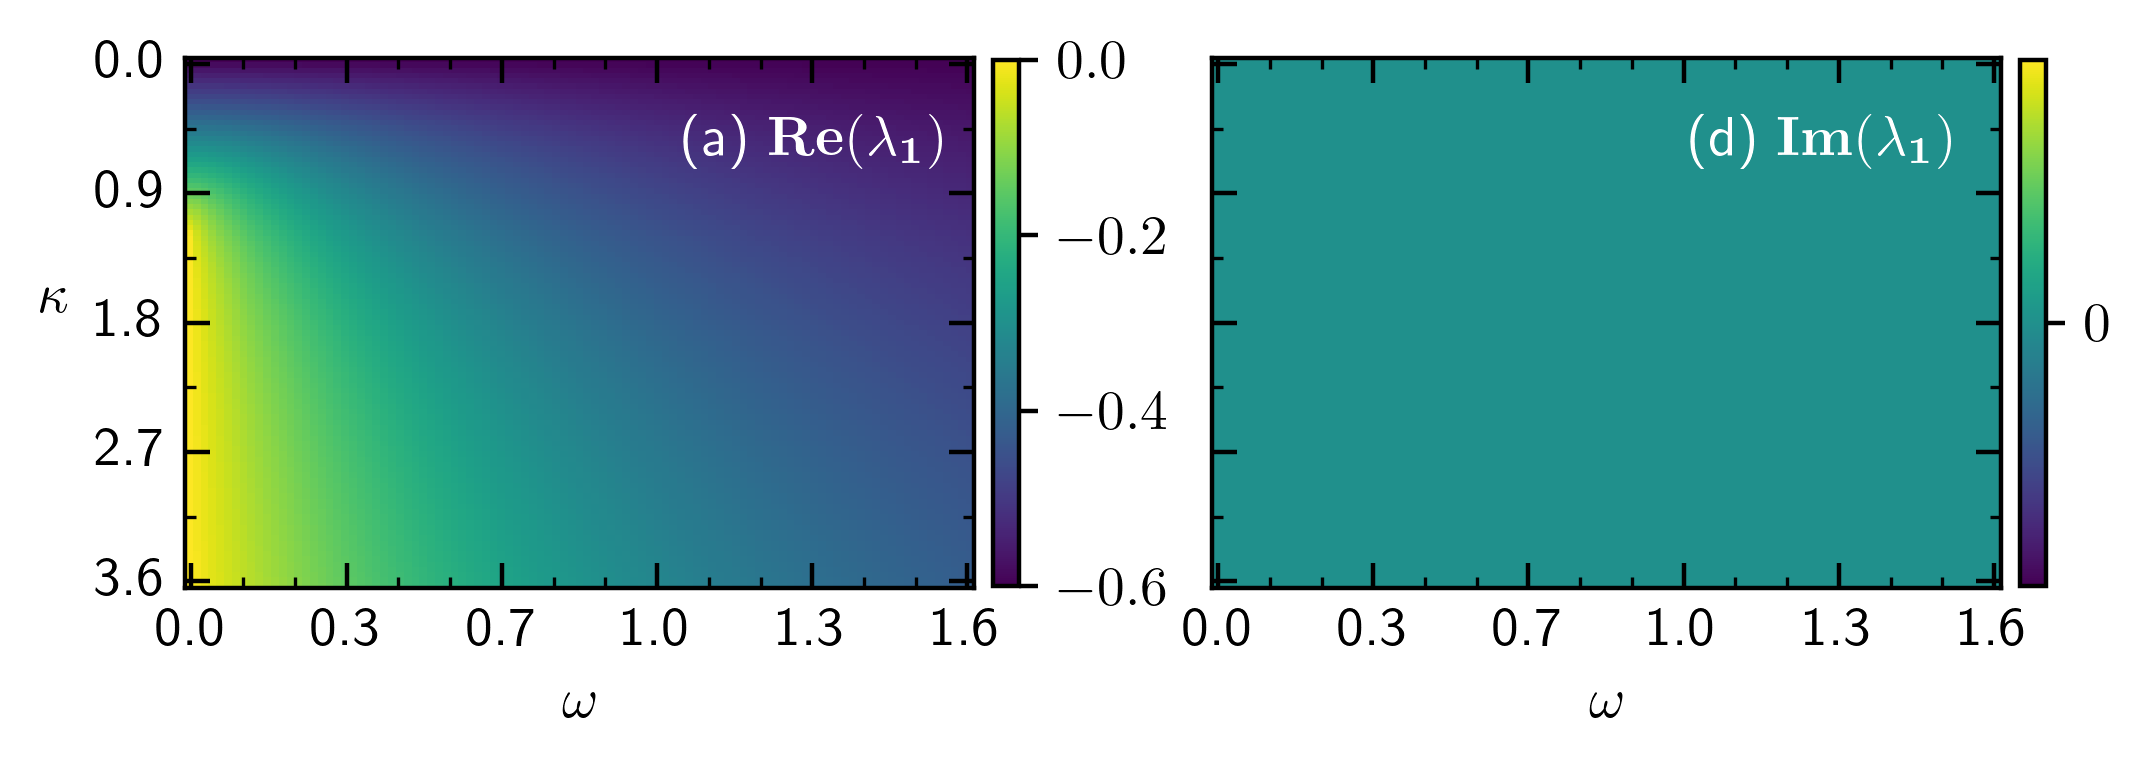
\includegraphics{pictures/lam_anal_s_1.png}
    \caption{In this graph the first eigenvalue of the fixed point with the smallest $y$-value are plotted.}
    \label{fig:eig_value_stab1}
\end{figure}
\begin{figure}[H]
    \centering
    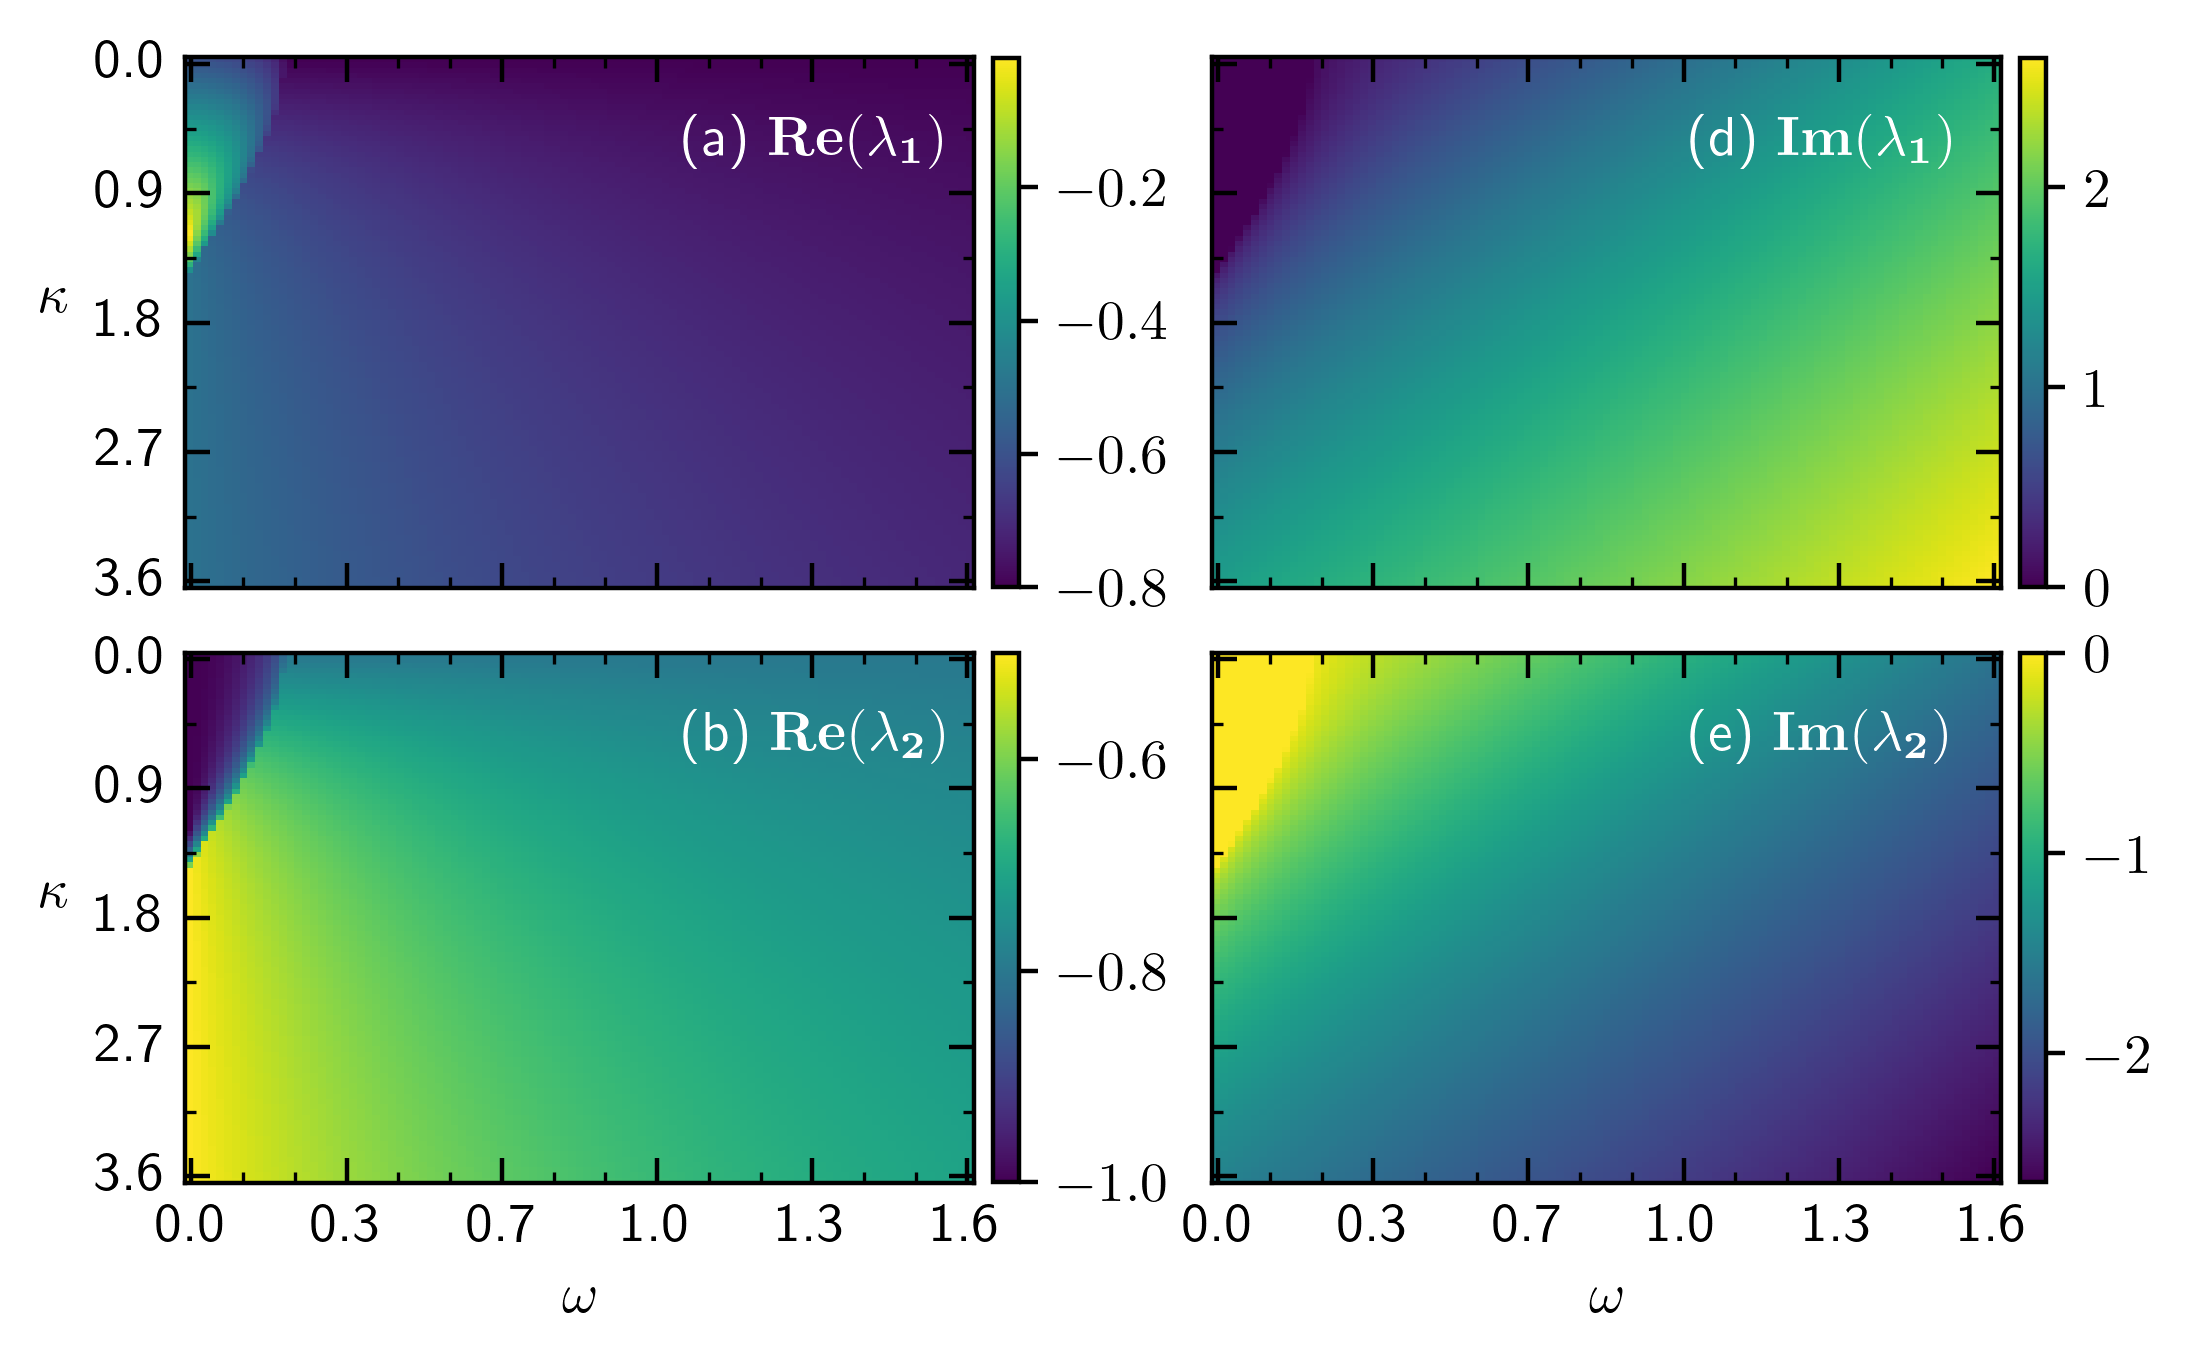
\includegraphics{pictures/lam_anal_s_2.png}
    \caption{In this graph the second and third eigenvalue of the fixed point with the smallest $y$-value are plotted. Notice the region of small $\kappa$ and $\omega$ in the top left corner of the real and imaginary parts of the eigenvalues. Here the real part changes rather quickly, which stems from the square root becoming real (\figref{fig:sign_lam23_s}).
    }
    \label{fig:eig_value_stab2}
\end{figure}

By studying the constraint of zero detuning, I was able to perform a good part of the characterization of that system analytically. This allowed to get an intuition on how changes in the equations of motion due to different parameter values can influence the existence and stability of fixed points. Without detuning I found that the system always decays to a stationary fixed point, indifferently whether there were 3 or 1 stationary solutions to the equation of motion. Nevertheless outsets of oscillatory dynamics have been observed, giving rise to the question, whether the onset of detuning can change the stability of those oscillations. 
